\section{Stateful action}\label{stateful-action}

Some actions have states. The typical values of states are boolean or
string. However, other types of states are possible if you want.

Actions which have states are called stateful.

\subsection{Stateful action without a
parameter}\label{stateful-action-without-a-parameter}

Some menus are called toggle menu. For example, fullscreen menu has a
state which has two values -- fullscreen and non-fullscreen. The value
of the state is changed every time the menu is clicked. An action
corresponds to the fullscreen menu also have a state. Its value is TRUE
or FALSE and it is called boolean value. TRUE corresponds to fullscreen
and FALSE to non-fullscreen.

The following is an example code to implement a fullscreen menu except
the signal handler. The signal handler will be shown later.

\begin{lstlisting}[language=C]
GSimpleAction *act_fullscreen = g_simple_action_new_stateful ("fullscreen",
                                NULL, g_variant_new_boolean (FALSE));
g_signal_connect (act_fullscreen, "change-state", G_CALLBACK (fullscreen_changed), win);
g_action_map_add_action (G_ACTION_MAP (win), G_ACTION (act_fullscreen));
... ... ...
GMenuItem *menu_item_fullscreen = g_menu_item_new ("Full Screen", "win.fullscreen");
\end{lstlisting}

\begin{itemize}
\tightlist
\item
  \passthrough{\lstinline!act\_fullscreen!} is a GSimpleAction instance.
  It is created with
  \passthrough{\lstinline!g\_simple\_action\_new\_stateful!}. The
  function has three arguments. The first argument ``fullscreen'' is the
  name of the action. The second argument is a parameter type.
  \passthrough{\lstinline!NULL!} means the action doesn't have a
  parameter. The third argument is the initial state of the action. It
  is a GVariant value. GVariant will be explained in the next
  subsection. The function
  \passthrough{\lstinline!g\_variant\_new\_boolean (FALSE)!} returns a
  boolean type GVariant value which is \passthrough{\lstinline!FALSE!}.
  If there are two or more top level windows, each window has its own
  \passthrough{\lstinline!act\_fullscreen!} action. So, the number of
  the actions is the same as the number of the windows.
\item
  The action \passthrough{\lstinline!act\_fullscreen!} has
  ``change-state'' signal. The signal is connected to a handler
  \passthrough{\lstinline!fullscreen\_changed!}. If the fullscreen menu
  is clicked, then the corresponding action
  \passthrough{\lstinline!act\_fullscreen!} is activated. But no handler
  is connected to the ``activate'' signal. Then, the default behavior
  for boolean-stated actions with a NULL parameter type like
  \passthrough{\lstinline!act\_fullscreen!} is to toggle them via the
  ``change-state'' signal.
\item
  The action is added to the GtkWindow \passthrough{\lstinline!win!}.
  Therefore, the scope of the action is ``win''.
\item
  \passthrough{\lstinline!menu\_item\_fullscreen!} is a GMenuItem
  instance. There are two arguments. The first argument ``Full Screen''
  is the label of \passthrough{\lstinline!menu\_item\_fullscreen!}. The
  second argument is an action. The action ``win.fullscreen'' has a
  prefix ``win'' and an action name ``fullscreen''. The prefix says that
  the action belongs to the window.
\end{itemize}

\begin{lstlisting}[language=C, numbers=left]
static void
fullscreen_changed(GSimpleAction *action, GVariant *value, GtkWindow *win) {
  if (g_variant_get_boolean (value))
    gtk_window_maximize (win);
  else
    gtk_window_unmaximize (win);
  g_simple_action_set_state (action, value);
}
\end{lstlisting}

\begin{itemize}
\tightlist
\item
  The handler \passthrough{\lstinline!fullscreen\_changed!} has three
  parameters. The first parameter is the action which emits the
  ``change-state'' signal. The second parameter is the value of the new
  state of the action. The third parameter is a user data which is set
  in \passthrough{\lstinline!g\_signal\_connect!}.
\item
  If the value is boolean type and \passthrough{\lstinline!TRUE!}, then
  it maximizes the window. Otherwise it un-maximizes.
\item
  Sets the state of the action with \passthrough{\lstinline!value!}.
  Note: At this stage, that means the stage before
  \passthrough{\lstinline!g\_simple\_action\_set\_state!} is called, the
  state of the action still has the original value. So, you need to set
  the state with the new value by
  \passthrough{\lstinline!g\_simple\_action\_set\_state!}.
\end{itemize}

You can use ``activate'' signal instead of ``change-state'' signal, or
both signals. But the way above is the simplest and the best.

\subsubsection{GVariant}\label{gvariant}

GVariant is a fundamental type. It isn't a child of GObject. GVariant
can contain boolean, string or other type values. For example, the
following program assigns TRUE to \passthrough{\lstinline!value!} whose
type is GVariant.

\begin{lstlisting}[language=C]
GVariant *value = g_variant_new_boolean (TRUE);
\end{lstlisting}

Another example is:

\begin{lstlisting}[language=C]
GVariant *value2 = g_variant_new_string ("Hello");
\end{lstlisting}

\passthrough{\lstinline!value2!} is a GVariant and it has a string type
value ``Hello''. GVariant can contain other types like int16, int32,
int64, double and so on.

If you want to get the original value, use g\_variant\_get series
functions. For example, you can get the boolean value with
g\_variant\_get\_boolean.

\begin{lstlisting}[language=C]
gboolean bool = g_variant_get_boolean (value);
\end{lstlisting}

Since \passthrough{\lstinline!value!} has been created as a boolean type
GVariant with \passthrough{\lstinline!TRUE!} value,
\passthrough{\lstinline!bool!} equals \passthrough{\lstinline!TRUE!}. In
the same way, you can get a string from \passthrough{\lstinline!value2!}

\begin{lstlisting}[language=C]
const char *str = g_variant_get_string (value2, NULL);
\end{lstlisting}

The second parameter is a pointer to gsize type variable (gsize is
defined as unsigned long). If it isn't NULL, then the pointed value is
used as the length by the function. If it is NULL, nothing happens. The
returned string \passthrough{\lstinline!str!} is owned by the instance
and can't be changed or freed by the caller.

\subsection{Stateful action with a
parameter}\label{stateful-action-with-a-parameter}

Another example of stateful actions is an action corresponds to color
select menus. For example, there are three menus and each menu has red,
green or blue color respectively. They determine the background color of
a GtkLabel widget. One action is connected to the three menus. The
action has a state whose value is ``red'', ``green'' or ``blue''. The
values are string. Those colors are given to the signal handler as a
parameter.

\begin{lstlisting}[language=C]
... ... ...
GVariantType *vtype = g_variant_type_new("s");
GSimpleAction *act_color
  = g_simple_action_new_stateful ("color", vtype, g_variant_new_string ("red"));
g_variant_type_free (vtype);
GMenuItem *menu_item_red = g_menu_item_new ("Red", "app.color::red");
GMenuItem *menu_item_green = g_menu_item_new ("Green", "app.color::green");
GMenuItem *menu_item_blue = g_menu_item_new ("Blue", "app.color::blue");
g_signal_connect (act_color, "activate", G_CALLBACK (color_activated), NULL);
... ... ...
\end{lstlisting}

\begin{itemize}
\tightlist
\item
  GVariantType is a C structure and it keeps a type of GVariant. It is
  created with the function
  \passthrough{\lstinline!g\_variant\_type\_new!}. The argument of the
  function is a GVariant type string. So,
  \passthrough{\lstinline!g\_variant\_type\_new("s")!} returns a
  GVariantType structure contains a string type. The returned value,
  GVariantType structure, is owned by the caller. So, you need to free
  it when it becomes useless.
\item
  The variable \passthrough{\lstinline!act\_color!} points a
  GSimpleAction instance. It is created with
  \passthrough{\lstinline!g\_simple\_action\_new\_stateful!}. The
  function has three arguments. The first argument ``color'' is the name
  of the action. The second argument is a parameter type which is
  GVariantType. \passthrough{\lstinline!g\_variant\_type\_new("s")!}
  creates GVariantType which is a string type
  (\passthrough{\lstinline!G\_VARIANT\_TYPE\_STRING!}). The third
  argument is the initial state of the action. It is a GVariant. The
  function \passthrough{\lstinline!g\_variant\_new\_string ("red")!}
  returns a GVariant value which has the string value ``red''. GVariant
  has a reference count and
  \passthrough{\lstinline!g\_variant\_new\_...!} series functions
  returns a GVariant value with a floating reference. That means the
  caller doesn't own the value at this point. And
  \passthrough{\lstinline!g\_simple\_action\_new\_stateful!} function
  consumes the floating reference so you don't need to care about
  releasing the GVariant instance.
\item
  The GVariantType structure \passthrough{\lstinline!vtype!} is useless
  after \passthrough{\lstinline!g\_simple\_action\_new\_stateful!}. It
  is released with the function
  \passthrough{\lstinline!g\_variant\_type\_free!}.
\item
  The varable \passthrough{\lstinline!menu\_item\_red!} points a
  GMenuItem instance. The function
  \passthrough{\lstinline!g\_menu\_item\_new!} has two arguments. The
  first argument ``Red'' is the label of
  \passthrough{\lstinline!menu\_item\_red!}. The second argument is a
  detailed action. Its prefix is ``app'', action name is ``color'' and
  target is ``red''. Target is sent to the action as a parameter. The
  same goes for \passthrough{\lstinline!menu\_item\_green!} and
  \passthrough{\lstinline!menu\_item\_blue!}.
\item
  The function \passthrough{\lstinline!g\_signal\_connect!} connects the
  activate signal on the action \passthrough{\lstinline!act\_color!} and
  the handler \passthrough{\lstinline!color\_activated!}. If one of the
  three menus is clicked, then the action
  \passthrough{\lstinline!act\_color!} is activated with the target
  (parameter) which is given by the menu.
\end{itemize}

The following is the ``activate'' signal handler.

\begin{lstlisting}[language=C]
static void
color_activated(GSimpleAction *action, GVariant *parameter) {
  char *color = g_strdup_printf ("label.lb {background-color: %s;}",
                                   g_variant_get_string (parameter, NULL));
  gtk_css_provider_load_from_data (provider, color, -1);
  g_free (color);
  g_action_change_state (G_ACTION (action), parameter);
}
\end{lstlisting}

\begin{itemize}
\tightlist
\item
  The handler originally has three parameters. The third parameter is a
  user data set in the \passthrough{\lstinline!g\_signal\_connect!}
  function. But it is left out because the fourth argument of the
  \passthrough{\lstinline!g\_signal\_connect!} has been NULL. The first
  parameter is the action which emits the ``activate'' signal. The
  second parameter is the parameter, or target, given to the action. It
  is a color specified by the menu.
\item
  The variable \passthrough{\lstinline!color!} is a CSS string created
  by \passthrough{\lstinline!g\_strdup\_printf!}. The arguments of
  \passthrough{\lstinline!g\_strdup\_printf!} are the same as printf C
  standard function. The function
  \passthrough{\lstinline!g\_variant\_get\_string!} gets the string
  contained in \passthrough{\lstinline!parameter!}. The string is owned
  by the instance and you mustn't change or free it. The string
  \passthrough{\lstinline!label.lb!} is a selector. It consists of
  \passthrough{\lstinline!label!}, a node name of GtkLabel, and
  \passthrough{\lstinline!lb!} which is a class name. It selects
  GtkLabel which has \passthrough{\lstinline!lb!} class. For example,
  menus have GtkLabel to display their labels, but they don't have
  \passthrough{\lstinline!lb!} class. So, the CSS doesn't change their
  background color. The string
  \passthrough{\lstinline!\{background-color \%s\}!} makes the
  background color \passthrough{\lstinline!\%s!} to which the color from
  \passthrough{\lstinline!parameter!} is assigned.
\item
  Frees the string \passthrough{\lstinline!color!}.
\item
  Changes the state with
  \passthrough{\lstinline!g\_action\_change\_state!}.
\end{itemize}

Note: If you haven't set an ``activate'' signal handler, the signal is
forwarded to ``change-state'' signal. So, you can use ``change-state''
signal instead of ``activate'' signal. See
\passthrough{\lstinline!src/menu/menu2\_change\_state.c!}.

\subsubsection{GVariantType}\label{gvarianttype}

GVariantType gives a type of GVariant. GVariantType is created with a
type string.

\begin{itemize}
\tightlist
\item
  ``b'' means boolean type.
\item
  ``s'' means string type.
\end{itemize}

The following program is a simple example. It finally outputs the string
``s''.

\begin{lstlisting}[language=C, numbers=left]
#include <glib.h>

int
main (int argc, char **argv) {
  GVariantType *vtype = g_variant_type_new ("s");
  const char *type_string = g_variant_type_peek_string (vtype);
  g_print ("%s\n",type_string);
  g_variant_type_free (vtype);
}
\end{lstlisting}

\begin{itemize}
\tightlist
\item
  The function \passthrough{\lstinline!g\_variant\_type\_new!} creates a
  GVariantType structure. The argument ``s'' is a type string. It means
  string. The returned structure is owned by the caller. When it becomes
  useless, you need to free it with the function
  \passthrough{\lstinline!g\_variant\_type\_free!}.
\item
  The function \passthrough{\lstinline!g\_variant\_type\_peek\_string!}
  takes a peek at \passthrough{\lstinline!vtype!}. It is the string
  ``s'' given to \passthrough{\lstinline!vtype!} when it was created.
  The string is owned by the instance and the caller can't change or
  free it.
\item
  Prints the string to the terminal. You can't free
  \passthrough{\lstinline!vtype!} before
  \passthrough{\lstinline!g\_print!} because the string
  \passthrough{\lstinline!type\_string!} is owned by
  \passthrough{\lstinline!vtype!}.
\item
  Frees \passthrough{\lstinline!vtype!}.
\end{itemize}

\subsection{Example}\label{example}

The following code includes stateful actions above. This program has
menus like this:

\begin{figure}
\centering
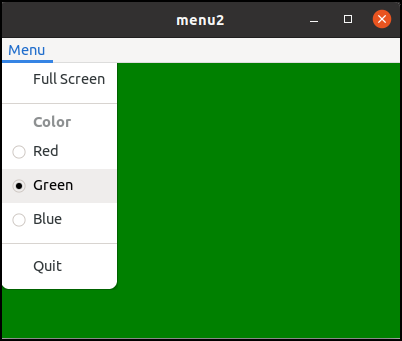
\includegraphics[width=6.03cm,height=5.115cm]{../image/menu2.png}
\caption{menu2}
\end{figure}

\begin{itemize}
\tightlist
\item
  Fullscreen menu toggles the size of the window between maximum and
  non-maximum. If the window is maximum size, which is called full
  screen, then a check mark is put before ``fullscreen'' label.
\item
  Red, green and blue menu determines the back ground color of the label
  in the window. The menus have radio buttons on the left of the menus.
  And the radio button of the selected menu turns on.
\item
  Quit menu quits the application.
\end{itemize}

The code is as follows.

\begin{lstlisting}[language=C, numbers=left]
#include <gtk/gtk.h>

/* The provider below provides application wide CSS data. */
GtkCssProvider *provider;

static void
fullscreen_changed(GSimpleAction *action, GVariant *value, GtkWindow *win) {
  if (g_variant_get_boolean (value))
    gtk_window_maximize (win);
  else
    gtk_window_unmaximize (win);
  g_simple_action_set_state (action, value);
}

static void
color_activated(GSimpleAction *action, GVariant *parameter) {
  char *color = g_strdup_printf ("label.lb {background-color: %s;}", g_variant_get_string (parameter, NULL));
  /* Change the CSS data in the provider. */
  /* Previous data is thrown away. */
  gtk_css_provider_load_from_data (provider, color, -1);
  g_free (color);
  g_action_change_state (G_ACTION (action), parameter);
}

static void
app_shutdown (GApplication *app, GtkCssProvider *provider) {
  gtk_style_context_remove_provider_for_display (gdk_display_get_default(), GTK_STYLE_PROVIDER (provider));
}

static void
app_activate (GApplication *app) {
  GtkWindow *win = GTK_WINDOW (gtk_application_window_new (GTK_APPLICATION (app)));
  gtk_window_set_title (win, "menu2");
  gtk_window_set_default_size (win, 400, 300);

  GtkWidget *lb = gtk_label_new (NULL);
  gtk_widget_add_css_class (lb, "lb"); /* the class is used by CSS Selector */
  gtk_window_set_child (win, lb);

  GSimpleAction *act_fullscreen
    = g_simple_action_new_stateful ("fullscreen", NULL, g_variant_new_boolean (FALSE));
  g_signal_connect (act_fullscreen, "change-state", G_CALLBACK (fullscreen_changed), win);
  g_action_map_add_action (G_ACTION_MAP (win), G_ACTION (act_fullscreen));

  gtk_application_window_set_show_menubar (GTK_APPLICATION_WINDOW (win), TRUE);

  gtk_window_present (win);
}

static void
app_startup (GApplication *app) {
  GVariantType *vtype = g_variant_type_new("s");
  GSimpleAction *act_color
    = g_simple_action_new_stateful ("color", vtype, g_variant_new_string ("red"));
  g_variant_type_free (vtype);
  GSimpleAction *act_quit
    = g_simple_action_new ("quit", NULL);
  g_signal_connect (act_color, "activate", G_CALLBACK (color_activated), NULL);
  g_signal_connect_swapped (act_quit, "activate", G_CALLBACK (g_application_quit), app);
  g_action_map_add_action (G_ACTION_MAP (app), G_ACTION (act_color));
  g_action_map_add_action (G_ACTION_MAP (app), G_ACTION (act_quit));

  GMenu *menubar = g_menu_new ();
  GMenu *menu = g_menu_new ();
  GMenu *section1 = g_menu_new ();
  GMenu *section2 = g_menu_new ();
  GMenu *section3 = g_menu_new ();
  GMenuItem *menu_item_fullscreen = g_menu_item_new ("Full Screen", "win.fullscreen");
  GMenuItem *menu_item_red = g_menu_item_new ("Red", "app.color::red");
  GMenuItem *menu_item_green = g_menu_item_new ("Green", "app.color::green");
  GMenuItem *menu_item_blue = g_menu_item_new ("Blue", "app.color::blue");
  GMenuItem *menu_item_quit = g_menu_item_new ("Quit", "app.quit");

  g_menu_append_item (section1, menu_item_fullscreen);
  g_menu_append_item (section2, menu_item_red);
  g_menu_append_item (section2, menu_item_green);
  g_menu_append_item (section2, menu_item_blue);
  g_menu_append_item (section3, menu_item_quit);
  g_object_unref (menu_item_red);
  g_object_unref (menu_item_green);
  g_object_unref (menu_item_blue);
  g_object_unref (menu_item_fullscreen);
  g_object_unref (menu_item_quit);

  g_menu_append_section (menu, NULL, G_MENU_MODEL (section1));
  g_menu_append_section (menu, "Color", G_MENU_MODEL (section2));
  g_menu_append_section (menu, NULL, G_MENU_MODEL (section3));
  g_menu_append_submenu (menubar, "Menu", G_MENU_MODEL (menu));
  g_object_unref (section1);
  g_object_unref (section2);
  g_object_unref (section3);
  g_object_unref (menu);

  gtk_application_set_menubar (GTK_APPLICATION (app), G_MENU_MODEL (menubar));

  provider = gtk_css_provider_new ();
  /* Initialize the css data */
  gtk_css_provider_load_from_data (provider, "label.lb {background-color: red;}", -1);
  /* Add CSS to the default GdkDisplay. */
  gtk_style_context_add_provider_for_display (gdk_display_get_default (),
        GTK_STYLE_PROVIDER (provider), GTK_STYLE_PROVIDER_PRIORITY_APPLICATION);
  g_signal_connect (app, "shutdown", G_CALLBACK (app_shutdown), provider);
  g_object_unref (provider); /* release provider, but it's still alive because the display owns it */
}

#define APPLICATION_ID "com.github.ToshioCP.menu2"

int
main (int argc, char **argv) {
  GtkApplication *app;
  int stat;

  app = gtk_application_new (APPLICATION_ID, G_APPLICATION_DEFAULT_FLAGS);
  g_signal_connect (app, "startup", G_CALLBACK (app_startup), NULL);
  g_signal_connect (app, "activate", G_CALLBACK (app_activate), NULL);

  stat =g_application_run (G_APPLICATION (app), argc, argv);
  g_object_unref (app);
  return stat;
}
\end{lstlisting}

\begin{itemize}
\tightlist
\item
  6-23: Action signal handlers.
\item
  25-28: The handler \passthrough{\lstinline!app\_shutdown!} is called
  when the application quits. It removes the provider from the display.
\item
  30-48: An activate signal handler.
\item
  32-34: A new window is created and assigned to
  \passthrough{\lstinline!win!}. Its title and default size are set to
  ``menu2'' and 400x300 respectively.
\item
  36-38: A new label is created and assigned to
  \passthrough{\lstinline!lb!} The label is given a CSS class ``lb''. It
  is added to \passthrough{\lstinline!win!} as a child.
\item
  40-43: A toggle action is created and assigned to
  \passthrough{\lstinline!act\_fullscreen!}. It's connected to the
  signal handler \passthrough{\lstinline!fullscreen\_changed!}. It's
  added to the window, so the action scope is ``win''. So, if there are
  two or more windows, the actions are created two or more.
\item
  45: The function
  \passthrough{\lstinline!gtk\_application\_window\_set\_show\_menubar!}
  adds a menubar to the window.
\item
  47: Shows the window.
\item
  50-104: A startup signal handler.
\item
  52-61: Two actions \passthrough{\lstinline!act\_color!} and
  \passthrough{\lstinline!act\_quit!} are created. These actions exists
  only one because the startup handler is called once. They are
  connected to their handlers and added to the application. Their scopes
  are ``app''.
\item
  63-92: Menus are built.
\item
  94: The menubar is added to the application.
\item
  96-103: A CSS provider is created with the CSS data and added to the
  default display. The ``shutdown'' signal on the application is
  connected to a handler ``app\_shutdown''. So, the provider is removed
  from the display and freed when the application quits.
\end{itemize}

\subsection{Compile}\label{compile}

Change your current directory to \passthrough{\lstinline!src/menu!}.

\begin{lstlisting}
$ comp menu2
$./a.out
\end{lstlisting}

Then, you will see a window and the background color of the content is
red. You can change the size to maximum and change back to the original
size. You can change the background color to green or blue.

If you run the second application during the first application is
running, another window will appear in the same screen. Both of the
window have the same background color. Because the
\passthrough{\lstinline!act\_color!} action has ``app'' scope and the
CSS is applied to the default display shared by the windows.

\begin{lstlisting}
$ ./a.out & # Run the first application
[1] 82113
$ ./a.out # Run the second application
$ 
\end{lstlisting}
